% Generated by book/tools/notebook_to_tex.py. Do not edit by hand.

\chapter[회귀 분석 (Regression \& MSE)]{회귀 분석 (Regression \& MSE)}

\label{ch:02}

\markboth{회귀 분석 (Regression \& MSE)}{회귀 분석 (Regression \& MSE)}

\chaptermeta{02_sklearn_regression/02_sklearn_regression.ipynb}{https://colab.research.google.com/github/yoon-gu/neuqes-101/blob/master/02_sklearn_regression/02_sklearn_regression.ipynb}{별점 예측을 통해 첫 손실인 평균제곱오차를 관찰}



\index{1Regression@Regression}

\index{1MSELoss@MSELoss}

\index{1LinearRegression@LinearRegression}

\index{1mean squared error@mean\_squared\_error}

\index{1Output Head@Output Head}

\index{0회귀@회귀}

\index{0평균제곱오차@평균제곱오차}

\index{0별점 예측@별점 예측}

\index{0비활성 출력@비활성 출력}

\index{0선형회귀@선형회귀}

\index{0정규방정식@정규방정식}

\index{0평균절대오차@평균절대오차}

\index{0결정계수@결정계수}

\index{1train test split@train\_test\_split}

\index{1mean absolute error@mean\_absolute\_error}

\index{1r2 score@r2\_score}

\index{1MAE@MAE}

\index{1R2 score@R2 score}

\index{1residual@residual}

\index{1prediction clipping@prediction clipping}

\index{1target normalization@target normalization}

\index{1np clip@np.clip}

\index{1regression head@regression head}

\index{1continuous target@continuous target}

\index{0잔차@잔차}

\index{0타깃 정규화@타깃 정규화}

\index{0예측값 클리핑@예측값 클리핑}

\index{0연속 타깃@연속 타깃}

\index{0회귀 헤드@회귀 헤드}

\index{0평가 지표@평가 지표}

\index{0과대 예측@과대 예측}

\index{0과소 예측@과소 예측}



\section{변화추적표}

\begin{booktable}{2장 변화추적표}{tab:ch02-01}
\begin{adjustbox}{max width=\textwidth}
\begin{tabular}{@{}lllllll@{}}
\toprule
Ch & 모델 & 토크나이저 & 데이터 & Output Head & Activation & Loss \\
\midrule

1 & (TF-IDF) & \inlinecode{TfidfVectorizer()} & Yelp 5,000 샘플 & --- & --- & --- \\
\textbf{2 \(\leftarrow\) 여기} & \inlinecode{LinearRegression()} & \inlinecode{TfidfVectorizer()} & Yelp (별점 1-5) & (1차원) & 없음 & \inlinecode{MSELoss} (sklearn: squared error) \\
\bottomrule
\end{tabular}
\end{adjustbox}
\end{booktable}

전체 장 표는 \href{https://github.com/yoon-gu/neuqes-101\#챕터별-변화추적표}{루트 README.md}를 참고하세요.



\section{변경점: \ref{ch:01}장 대비}

\begin{booktable}{2장 변경점 요약}{tab:ch02-02}
\begin{adjustbox}{max width=\textwidth}
\begin{tabular}{@{}lll@{}}
\toprule
축 & \ref{ch:01}장 & \ref{ch:02}장 \\
\midrule

모델 & 없음 (변환만) & \textbf{\inlinecode{LinearRegression}} \(\leftarrow\) 추가 \\
Loss & 없음 & \textbf{\inlinecode{MSELoss}} \(\leftarrow\) 첫 등장 \\
토크나이저 & TF-IDF & TF-IDF (그대로) \\
데이터 & Yelp 5,000 & Yelp 5,000 (그대로) \\
\bottomrule
\end{tabular}
\end{adjustbox}
\end{booktable}

이 장에서 바뀌는 것은 \textbf{모델 + Loss} 두 가지입니다 --- 그러나 둘은 한 묶음으로 처음 등장하는 거라, 학습자 관점에선 사실상 “모델이 처음 생겼다”는 한 가지 변화입니다. 다음 장부터는 한 번에 하나씩 변합니다.

\textbf{왜 회귀부터?} 모델이 출력하는 출력은 본질적으로 비활성 스칼라 출력입니다. 분류·다중라벨·multi-task 같은 복합적인 형태들은 모두 “그 숫자를 어떻게 가공해서 어떤 loss를 매길 것인가”의 변주일 뿐입니다. 가장 단순한 형태 --- 활성화 함수도 없는 1차원 출력 --- 부터 시작합니다.



\section{\texorpdfstring{손실 함수의 변화 --- 평균제곱오차 등장}{손실 함수의 변화 --- 평균제곱오차 등장}}

이 장의 loss는 \textbf{Mean Squared Error} 입니다.

\begin{equation}
\label{eq:ch02-01}
L = \frac{1}{N} \sum_{i=1}^{N} (y_i - \hat y_i)^2
\end{equation}

식~\eqref{eq:ch02-01}은 회귀에서 사용하는 Mean Squared Error의 정의입니다.

\begin{itemize}
\tightlist
\item
  \(y_i\): 정답 (정답 별점)
\item
  \(\hat y_i\): 모델 예측
\end{itemize}

\textbf{숫자로 감 잡기} (정답이 별점 5인 한 샘플 기준, \(N=1\)이라 평균은 그대로):

\begin{booktable}{2장 손실 함수의 변화 - 평균제곱오차 등장 표}{tab:ch02-03}
\begin{adjustbox}{max width=\textwidth}
\begin{tabular}{@{}llll@{}}
\toprule
정답 \(y\) & 예측 \(\hat y\) & 오차 \(\vert{}y - \hat y\vert{}\) & 손실 \((y - \hat y)^2\) \\
\midrule

5 & 4 & 1 & \textbf{1} \\
5 & 3 & 2 & \textbf{4} \\
5 & 1 & 4 & \textbf{16} \\
\bottomrule
\end{tabular}
\end{adjustbox}
\end{booktable}

오차가 2배가 되면 손실은 4배, 4배가 되면 16배로 \textbf{비선형으로} 증폭됩니다. 이 제곱 항이 MSE의 성격을 결정합니다 --- “조금씩 자주 틀리는 것” 보다 “어쩌다 크게 틀리는 것”을 모델이 더 강하게 회피합니다.

PyTorch에서는 \inlinecode{nn.MSELoss}, sklearn에서는 같은 개념이 \inlinecode{LinearRegression}에 내장돼 있고 평가 함수로는 \inlinecode{mean\_squared\_error}로 따로 부릅니다.

\Needspace{9\baselineskip}
\begin{lstlisting}
criterion = nn.MSELoss()
loss = criterion(pred, target)

from sklearn.linear_model import LinearRegression
from sklearn.metrics import mean_squared_error
model.fit(X, y)
mean_squared_error(y, model.predict(X))
\end{lstlisting}



\section{토크나이저 노트}

이 장의 토크나이저는 \textbf{\ref{ch:01}장과 동일한 \inlinecode{TfidfVectorizer}} 입니다. 변하는 건 그 위에 모델이 붙는다는 것뿐이라, 같은 입력 벡터에서 출발해 모델만 차이를 만들도록 합니다.

같은 문장 \inlinecode{"I\ love\ using\ Hugging\ Face!"} 의 토큰화 결과는 \ref{ch:01}장과 똑같습니다 --- 소문자, 단일 문자 제거, OOV 무시. 모델 입장에서 입력은 길이 V짜리 sparse 벡터 한 개고, 그걸 받아 \textbf{숫자 한 개} 를 출력하면 됩니다.

\begin{previewBox}{미리보기}
\textbf{다음 장(\ref{ch:03}장)}: 같은 TF-IDF 그대로. 변하는 건 출력에 sigmoid가 붙고 loss가 \inlinecode{BCEWithLogitsLoss}로 바뀌는 것입니다.
\end{previewBox}



\section{실습: 별점 1-5를 그대로 회귀하기}

\inlinecode{LinearRegression}은 가중치 벡터 \(w\)와 편향 \(b\)를 학습해 다음을 출력합니다.

\begin{equation}
\label{eq:ch02-02}
\hat y = w^\top x + b
\end{equation}

식~\eqref{eq:ch02-02}은 선형 모델의 출력이 특성 벡터와 가중치의 선형 결합임을 나타냅니다.

활성화 함수 없음, 출력 범위 제한 없음. 정답 \(y\)와의 MSE를 최소화하도록 \(w, b\)를 푸는 게 학습의 전부입니다 (sklearn은 정규방정식으로 한 번에 풉니다).



\Needspace{11\baselineskip}
\begin{lstlisting}
model = LinearRegression()
model.fit(X_train, y_train)

y_pred_train = model.predict(X_train)
y_pred_test = model.predict(X_test)

print(
    f"Train MSE: "
    f"{mean_squared_error(y_train, y_pred_train):.4f}"
)
print(
    f"Test  MSE: "
    f"{mean_squared_error(y_test,  y_pred_test):.4f}"
)
print(
    f"Test  MAE: "
\end{lstlisting}

\noindent\emph{앞 블록은 모델 출력을 확률이나 예측값으로 바꾸는 단계입니다. 이어지는 블록에서는 앞에서 만든 중간 값을 다음 계산으로 넘기는 단계로 넘어갑니다.}

\Needspace{5\baselineskip}
\begin{lstlisting}[firstnumber=17]
    f"{mean_absolute_error(y_test, y_pred_test):.4f}"
)
print(f"Test  R²:  {r2_score(y_test, y_pred_test):.4f}")
\end{lstlisting}

\begin{codeRead}
\textbf{1행}의 \inlinecode{model = ...}에서는 이번 실습에서 관찰할 모델 객체를 정의합니다. \textbf{2행}의 \inlinecode{model.fit(...)}에서는 학습 데이터로 모델 또는 변환기를 적합합니다. \textbf{4행}의 \inlinecode{y\_pred\_train = ...}에서는 학습된 모델로 최종 예측값을 만듭니다.
\end{codeRead}

\noindent\textbf{출력.}
\begin{bookoutputbox}
Train MSE: 0.0000
Test  MSE: 1.5565
Test  MAE: 0.9952
Test  R²:  0.2139
\end{bookoutputbox}
\par\vspace{0.9em}



\compactCodeOmitted{숫자 결과를 그림으로 확인하는 단계}

\begin{bookfigurelabel}[H]{회귀 예측값과 실제 별점 분포}{fig:ch02-prediction-distribution}
\centering
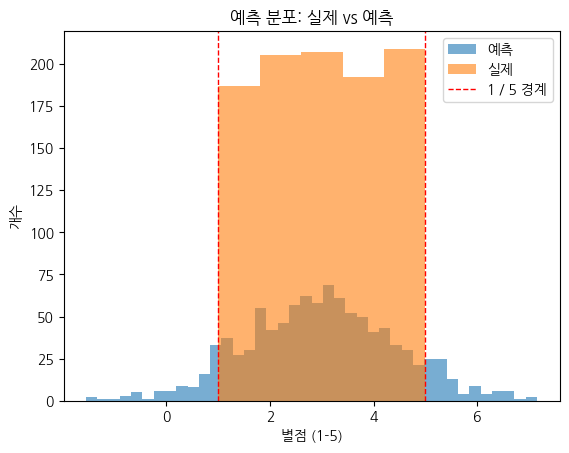
\includegraphics[width=0.76\linewidth]{assets/figures/ch02_prediction_distribution.png}
\end{bookfigurelabel}

\textbf{그림 읽기} --- 그림~\ref{fig:ch02-prediction-distribution}에서 다음 내용을 확인합니다: 회귀 예측값과 실제 별점 분포. 실행된 노트북에서 저장된 최신 plot 출력이므로, 코드에서 계산한 값이 어떤 평가 지점으로 이어지는지 바로 확인할 수 있습니다.



\section{해부: “출력은 비활성 스칼라 출력입니다”}

위 분포를 보면 모델이 0.4점이나 5.7점 같은 \textbf{별점 범위 밖} 의 값도 출력합니다. 이상해 보이지만 자연스러운 결과입니다.

\inlinecode{LinearRegression}이 학습한 것은 단지 “MSE를 최소화하는 가중합”이지, “출력값이 1과 5 사이여야 한다”는 제약을 포함하지 않습니다. 모델은 활성화 함수 없이 \(w^\top x + b\)를 그대로 출력할 뿐이라 음수도 5 초과도 모두 가능한 결과입니다.

이게 \textbf{회귀의 본질} 입니다. 출력 범위 제약은 모델이 아니라 사람이 따로 입혀야 합니다 --- clipping 같은 후처리, 혹은 sigmoid 같은 활성화 함수로요.



\section{변형: 별점을 {[}0, 1{]}로 정규화}

회귀의 출력이 어차피 임의 범위를 갖는다면, 정답 라벨을 일부러 {[}0, 1{]}로 정규화하면 어떻게 될까요? 별점 1-5를 4로 나눠 {[}0, 1{]} 사이로 압축합니다.

\begin{equation}
\label{eq:ch02-03}
y' = \frac{y - 1}{4} \in [0, 1]
\end{equation}

식~\eqref{eq:ch02-03}은 이 절에서 사용하는 핵심 관계를 정리한 것입니다.

이게 의미 있는 이유는 \textbf{다음 장의 다리} 가 되기 때문입니다. \ref{ch:03}장에서 sigmoid를 출력에 붙여 강제로 {[}0, 1{]}로 누를 텐데, 그때 정답 라벨도 {[}0, 1{]} 형식이어야 호환됩니다.



\Needspace{11\baselineskip}
\begin{lstlisting}
y_train_norm = (y_train - 1) / 4   # 1-5 -> 0-1
y_test_norm = (y_test - 1) / 4

model_norm = LinearRegression()
model_norm.fit(X_train, y_train_norm)

y_pred_norm = model_norm.predict(X_test)

print(
    f"Test MSE (normalized space): "
    f"{mean_squared_error(y_test_norm, y_pred_norm):.4f}"
)

\end{lstlisting}

\noindent\emph{앞 블록은 모델 출력을 확률이나 예측값으로 바꾸는 단계입니다. 이어지는 블록에서는 앞에서 만든 중간 값을 다음 계산으로 넘기는 단계로 넘어갑니다.}

\Needspace{11\baselineskip}
\begin{lstlisting}[firstnumber=14]
y_pred_back = y_pred_norm * 4 + 1
print(
    f"Test MSE (back to star space): "
    f"{mean_squared_error(y_test, y_pred_back):.4f}"
)
print(
    f"Test MSE (no normalization):    "
    f"{mean_squared_error(y_test, y_pred_test):.4f}"
)
\end{lstlisting}

\noindent\textbf{출력.}
\begin{bookoutputbox}
Test MSE (normalized space): 0.0973
Test MSE (back to star space): 1.5565
Test MSE (no normalization):    1.5565
\end{bookoutputbox}
\par\vspace{0.9em}



\textbf{관찰}: 정답 라벨을 {[}0, 1{]}로 압축해도 모델 출력은 여전히 그 범위를 벗어납니다. 가중합을 그대로 출력하는 한 어떤 라벨 스케일링으로도 {[}0, 1{]} 안에 가둘 수 없습니다.

그렇다면 출력을 강제로 {[}0, 1{]} 사이로 누르려면 \textbf{활성화 함수} 가 필요합니다.

\begin{previewBox}{미리보기}
\textbf{다음 장(\ref{ch:03}장) 예고}: \inlinecode{LogisticRegression}이 등장합니다. 모델 구조는 대부분 동일하게지만 출력층 직전에 \textbf{sigmoid} 가 붙어 {[}0, 1{]}을 강제하고, loss는 MSE 대신 \textbf{\inlinecode{BCEWithLogitsLoss}} (sklearn: log loss)로 바뀝니다. 라벨도 {[}0, 1{]} 정규화 대신 \textbf{0/1 이진} 으로 바뀝니다.
\end{previewBox}



\section{이 장에 등장한 라이브러리}

\begin{booktable}{2장 새로 등장한 라이브러리}{tab:ch02-04}
\begin{adjustbox}{max width=\textwidth}
\begin{tabular}{@{}lll@{}}
\toprule
이름 & 한 줄 설명 & 다음 장에서 \\
\midrule

\inlinecode{sklearn.linear\_model.LinearRegression} & MSE 최소화 1차원 회귀 & sklearn 모델 라인업의 시작, BERT는 \ref{ch:08}장부터 같은 역할 \\
\inlinecode{sklearn.model\_selection.train\_test\_split} & 훈련/평가 분할 & \ref{ch:03}--\ref{ch:05}장에서 계속 사용 \\
\inlinecode{sklearn.metrics.mean\_squared\_error} & MSE 평가 & \ref{ch:08}장 BERT 회귀에서도 평가 지표로 등장 \\
\inlinecode{sklearn.metrics.mean\_absolute\_error} & MAE 평가 (참고용) & --- \\
\inlinecode{sklearn.metrics.r2\_score} & 결정계수 R² & --- \\
\bottomrule
\end{tabular}
\end{adjustbox}
\end{booktable}



\section{체크포인트 질문}

\begin{enumerate}
\def\labelenumi{\arabic{enumi}.}
\tightlist
\item
  \inlinecode{LinearRegression}은 왜 활성화 함수가 없나요? 회귀에서 활성화 함수가 빠지면 어떤 자유도가 생기나요?
\item
  MSE를 수식으로 적어보세요. 큰 오차에 큰 페널티를 주는 이유는 어느 항에서 오나요?
\item
  별점을 {[}0, 1{]}로 정규화한 모델의 예측값이 여전히 그 범위를 벗어나는 이유는 무엇인가요?
\item
  같은 데이터를 정규화 없이 학습한 모델과 정규화 후 학습한 모델은 (후처리로 되돌렸을 때) Test MSE가 거의 같습니다. 왜 그런가요?
\end{enumerate}



\section{FAQ}

\begin{faqBox}{Q1. (이론) MSE 대신 MAE를 쓰면 어떻게 다른가요?}

MSE는 오차를 제곱하지만 MAE(Mean Absolute Error)는 절댓값만 취합니다.

\begin{equation}
\label{eq:ch02-04}
\text{MSE} = \frac{1}{N}\sum (y_i - \hat y_i)^2 \qquad \text{MAE} = \frac{1}{N}\sum \vert{}y_i - \hat y_i\vert{}
\end{equation}

식~\eqref{eq:ch02-04}은 회귀에서 사용하는 Mean Squared Error의 정의입니다.

차이는 두 가지입니다.

\begin{enumerate}
\def\labelenumi{\arabic{enumi}.}
\tightlist
\item
  \textbf{outlier 민감도}: MSE는 큰 오차를 제곱해 압도적으로 큰 페널티를 주므로 outlier 한 개가 모델 전체를 끌어당깁니다. MAE는 선형이라 outlier에 덜 민감합니다 (robust).
\item
  \textbf{gradient 형태}: MSE의 gradient는 \(\hat y - y\) (오차에 비례), MAE는 \(\pm 1\) (오차와 무관한 상수). 그래서 SGD 기반 학습에서 MAE는 미세 조정이 어려울 수 있고 0 근처에서 비미분(non-differentiable)이라 변형(Huber loss 등)이 자주 쓰입니다.
\end{enumerate}

\Needspace{5\baselineskip}
\begin{lstlisting}
from sklearn.metrics import mean_absolute_error
mean_absolute_error(y_test, y_pred_test)
\end{lstlisting}

\end{faqBox}




\begin{faqBox}{Q5. (실무) 예측값이 5보다 크거나 1보다 작게 나오는데 어떻게 하나요?}

세 가지 선택지가 있습니다.

\begin{enumerate}
\def\labelenumi{\arabic{enumi}.}
\tightlist
\item
  \textbf{그대로 둔다 (가장 흔함)}: 평가 지표(MSE, MAE)는 범위 밖 값도 그대로 받습니다. 회귀에서는 범위 이탈을 굳이 막지 않는 게 일반적.
\item
  \textbf{clip으로 잘라낸다}: 후처리로 {[}1, 5{]} 안으로 강제.
\end{enumerate}

\Needspace{7\baselineskip}
\begin{lstlisting}
y_pred_clipped = np.clip(y_pred_test, 1, 5)
print(
    f"Test MSE (clip 후): "
    f"{mean_squared_error(y_test, y_pred_clipped):.4f}"
)
\end{lstlisting}

\begin{enumerate}
\def\labelenumi{\arabic{enumi}.}
\setcounter{enumi}{2}
\tightlist
\item
  \textbf{출력에 sigmoid를 붙인다}: 다음 장의 방법. 활성화 함수로 모델 단계에서 {[}0, 1{]}을 강제.
\end{enumerate}

선택은 목적에 따릅니다 --- UI에 보여줄 점수면 clip이 명확하고, 다른 모델과 합쳐 학습 신호로 쓸 거면 그대로 둡니다.

\end{faqBox}

\begin{faqBox}{Q6. (이론) 별점은 1, 2, 3, 4, 5의 정수인데 회귀로 다루는 게 맞나요? 분류가 더 낫지 않나요?}

둘 다 가능하고, 절대 정답은 없습니다.

\begin{itemize}
\tightlist
\item
  \textbf{회귀가 자연스러운 이유}: 별점은 \textbf{순서(ordinal)} 가 있습니다. 4점과 5점이 가깝다는 정보를 회귀는 보존합니다 (loss가 거리 기반).
\item
  \textbf{분류가 자연스러운 이유}: 클래스 사이 간격이 균등하지 않을 수 있습니다. 1점과 2점의 차이, 4점과 5점의 차이가 같은 의미일까요? 사람마다 다릅니다. 분류는 클래스 간 거리를 가정하지 않습니다.
\end{itemize}

이 커리큘럼에서는 두 관점을 모두 보여줍니다 --- \ref{ch:02}장 (회귀) \(\to\) \ref{ch:05}장 (5클래스 분류). 같은 데이터를 두 방식으로 다룰 때 결과가 어떻게 달라지는지 비교하면 회귀와 분류의 차이가 구체적으로 이해할 수 있습니다.
\end{faqBox}



\compactFAQMore{3}

\section{오류 실험 (선택)}

다음 코드를 돌려보고, 두 모델의 결과가 같은지 다른지 예측해보세요.

\Needspace{11\baselineskip}
\begin{lstlisting}
model_a = LinearRegression().fit(X_train, y_train)

model_b = LinearRegression().fit(X_train, y_train * 100)

pred_a = model_a.predict(X_test)
pred_b = model_b.predict(X_test) / 100

print(
    f"A vs B 예측 차이 최대: "
    f"{np.abs(pred_a - pred_b).max():.2e}"
)
\end{lstlisting}

힌트: 닫힌 형태 풀이에서 라벨에 상수를 곱하면 가중치도 같은 비율로 바뀔 뿐, 예측을 같은 스케일로 되돌리면 정확히 같은 값이 나와야 합니다.



\begin{previewBox}{미리보기: 다음 장}

\textbf{\ref{ch:03}장. 이진 분류 (Binary Classification \& BCE) --- 출력에 sigmoid가 붙다}

\begin{itemize}
\tightlist
\item
  별점을 4-5점 \(\to\) 1, 1-2점 \(\to\) 0으로 이진화 (3점은 제외)
\item
  \inlinecode{LogisticRegression}: 출력에 \textbf{sigmoid} 가 붙고, loss는 \textbf{\inlinecode{BCEWithLogitsLoss}} (sklearn: log loss)로 바뀜
\item
  처음으로 “확률”을 출력하는 모델 --- \inlinecode{predict\_proba}로 확인
\item
  변경점은 \textbf{출력 형태 + Loss} 두 가지 (모델·토크나이저는 그대로, 데이터는 이진화로 가공)
\end{itemize}
\end{previewBox}